% !TEX program = xelatex
% Copyright 2004 by Till Tantau <tantau@users.sourceforge.net>.
%
% In principle, this file can be redistributed and/or modified under
% the terms of the GNU Public License, version 2.
%
% However, this file is supposed to be a template to be modified
% for your own needs. For this reason, if you use this file as a
% template and not specifically distribute it as part of a another
% package/program, I grant the extra permission to freely copy and
% modify this file as you see fit and even to delete this copyright
% notice. 

\documentclass[x11names]{beamer}
\usepackage{multicol}
%\usepackage[colorlinks=false]{hyperref}
\graphicspath{{figures/}}
\bibliographystyle{apalike}
\usepackage{paralist}
\usepackage{cases}
\usepackage{booktabs}
\usepackage{tikz}
\usepackage{overpic}
\usetikzlibrary{mindmap,shapes,arrows,chains,shadows,decorations.markings}
%\usepackage{verbatim}
%\usepackage[active,tightpage]{preview}
%\PreviewEnvironment{tikzpicture}
%\setlength\PreviewBorder{5mm}%
\colorlet{lcfree}{Green3}
\colorlet{lcnorm}{Blue3}
\colorlet{lccong}{Red3}
% -------------------------------------------------
% Set up a new layer for the debugging marks, and make sure it is on
% top
\pgfdeclarelayer{marx}
\pgfsetlayers{main,marx}
% A macro for marking coordinates (specific to the coordinate naming
% scheme used here). Swap the following 2 definitions to deactivate
% marks.
\providecommand{\cmark}[2][]{%
  \begin{pgfonlayer}{marx}
    \node [nmark] at (c#2#1) {#2};
  \end{pgfonlayer}{marx}
  } 
\providecommand{\cmark}[2][]{\relax} 

% There are many different themes available for Beamer. A comprehensive
% list with examples is given here:
% http://deic.uab.es/~iblanes/beamer_gallery/index_by_theme.html
% You can uncomment the themes below if you would like to use a different
% one:
%\usetheme{AnnArbor}
%\usetheme{Antibes}
%\usetheme{Bergen}
\usetheme[hideothersubsections]{Berkeley}
%\usetheme{Berlin}
%\usetheme{Boadilla}
%\usetheme{boxes}
%\usetheme{CambridgeUS}
%\usetheme{Copenhagen}
%\usetheme{Darmstadt}
%\usetheme{default}
%\usetheme{Frankfurt}
%\usetheme{Goettingen}
%\usetheme{Hannover}
%\usetheme{Ilmenau}
%\usetheme{JuanLesPins}
%\usetheme{Luebeck}
%\usetheme{Madrid}
%\usetheme{Malmoe}
%\usetheme{Marburg}
%\usetheme{Montpellier}
%\usetheme{PaloAlto}
%\usetheme{Pittsburgh}
%\usetheme{Rochester}
%\usetheme{Singapore}
%\usetheme{Szeged}
%\usetheme{Warsaw}

% 手动添加底行作者、标题和日期。
\setbeamertemplate{footline}{%
  \leavevmode%
  \hbox{%
    \begin{beamercolorbox}[wd=.4\paperwidth,ht=2.25ex,dp=1ex,center]{author in head/foot}%
      \usebeamerfont{author in head/foot}\insertshortauthor
    \end{beamercolorbox}%
    \begin{beamercolorbox}[wd=.3\paperwidth,ht=2.25ex,dp=1ex,center]{title in head/foot}%
      \usebeamerfont{title in head/foot}\insertshorttitle
    \end{beamercolorbox}%
    \begin{beamercolorbox}[wd=.3\paperwidth,ht=2.25ex,dp=1ex,right]{date in head/foot}%
      \usebeamerfont{date in head/foot}\today{}\hspace*{2em}
      \insertframenumber{} / \inserttotalframenumber\hspace*{2ex}
    \end{beamercolorbox}}%
  \vskip0pt%
}
%%%%%%%%%%%%%%%%%%%%%%%%%%

% sidebar 字体大小的调整。
%\setbeamerfont{section in sidebar}{size=\fontsize{2}{4}\selectfont}
%\setbeamerfont{subsection in sidebar}{size=\fontsize{2}{4}\selectfont}
%\setbeamerfont{subsubsection in sidebar}{size=\fontsize{2}{4}\selectfont}
%%%%%%%%%%%%%%%%%%%%%%%%%%%%%%%%%%%%%



\title{Cloud Manufacturing Ecosystem}

% A subtitle is optional and this may be deleted
\subtitle{Scheduling and Evolving}

\author{\href{mailto:42@zju.edu.cn}{Chen Shengkai}} %\inst{1} 
  %\and S.~Another\inst{2}

% - Give the names in the same order as the appear in the paper.
% - Use the \inst{?} command only if the authors have different
%   affiliation.

\institute[Zhejiang University] % (optional, but mostly needed)
{
  %\inst{1}
  Institute for Manufacturing Engineering and Automation\\
  Zhejiang University%\\
  %\href{mailto:42@zju.edu.cn}{42@zju.edu.cn}
%  \and
%  \inst{2}%
%  Department of Theoretical Philosophy\\
%  University of Elsewhere}
}
% - Use the \inst command only if there are several affiliations.
% - Keep it simple, no one is interested in your street address.

\date{INFORMS Annual Meeting, 2015}
% - Either use conference name or its abbreviation.
% - Not really informative to the audience, more for people (including
%   yourself) who are reading the slides online

% logo
\logo{
\includegraphics[scale = 0.2]{QSY.pdf}} % you can % i
%

\subject{Cloud Manufacturing}
% This is only inserted into the PDF information catalog. Can be left
% out. 

% If you have a file called "university-logo-filename.xxx", where xxx
% is a graphic format that can be processed by latex or pdflatex,
% resp., then you can add a logo as follows:

% \pgfdeclareimage[height=0.5cm]{university-logo}{university-logo-filename}
% \logo{\pgfuseimage{university-logo}}

% Delete this, if you do not want the table of contents to pop up at
% the beginning of each subsection:
%\iffalse
\AtBeginSubsection[]
{
  \begin{frame}<beamer>{Outline}
    \begin{multicols}{2}
    \tableofcontents[currentsection,currentsubsection]
    \end{multicols}
  \end{frame}
  \addtocounter{framenumber}{-1}
}
%\fi
% Let's get started
\begin{document}

\begin{frame}
  \titlepage
\end{frame}

\begin{frame}{Outline}
  \begin{multicols}{2}
  \tableofcontents
  \end{multicols}
  % You might wish to add the option [pausesections]
\end{frame}

% Section and subsections will appear in the presentation overview
% and table of contents.
% !TEX root = ../beamer.tex
\section{Introduction and Preliminary}

\subsection{Our Projects}

\begin{frame}{Introduction}{Our Projects}
  \begin{itemize}
  \item {
    My first point.
  }
  \item {
    My second point.
  }
  \end{itemize}
\end{frame}


\subsection{Operating Mode}

% You can reveal the parts of a slide one at a time
% with the \pause command:
\begin{frame}{Preliminary}{Operating Mode}
  \begin{itemize}
  \item {
    First item.
    \pause % The slide will pause after showing the first item
  }
  \item {   
    Second item.
  }
  % You can also specify when the content should appear
  % by using <n->:
  \item<3-> {
    Third item.
  }
  \item<4-> {
    Fourth item.
  }
  % or you can use the \uncover command to reveal general
  % content (not just \items):
  \item<5-> {
    Fifth item. \uncover<6->{Extra text in the fifth item.}
  }
  \end{itemize}
\end{frame}


% !TEX root = ../beamer.tex
\section{Preliminary}

\subsection{Cloud Manufacturing}
\begin{frame}{Ecosystem Main Structure}{Cloud Manufacturing}
\only<1>{
	\begin{figure}
	\centering
	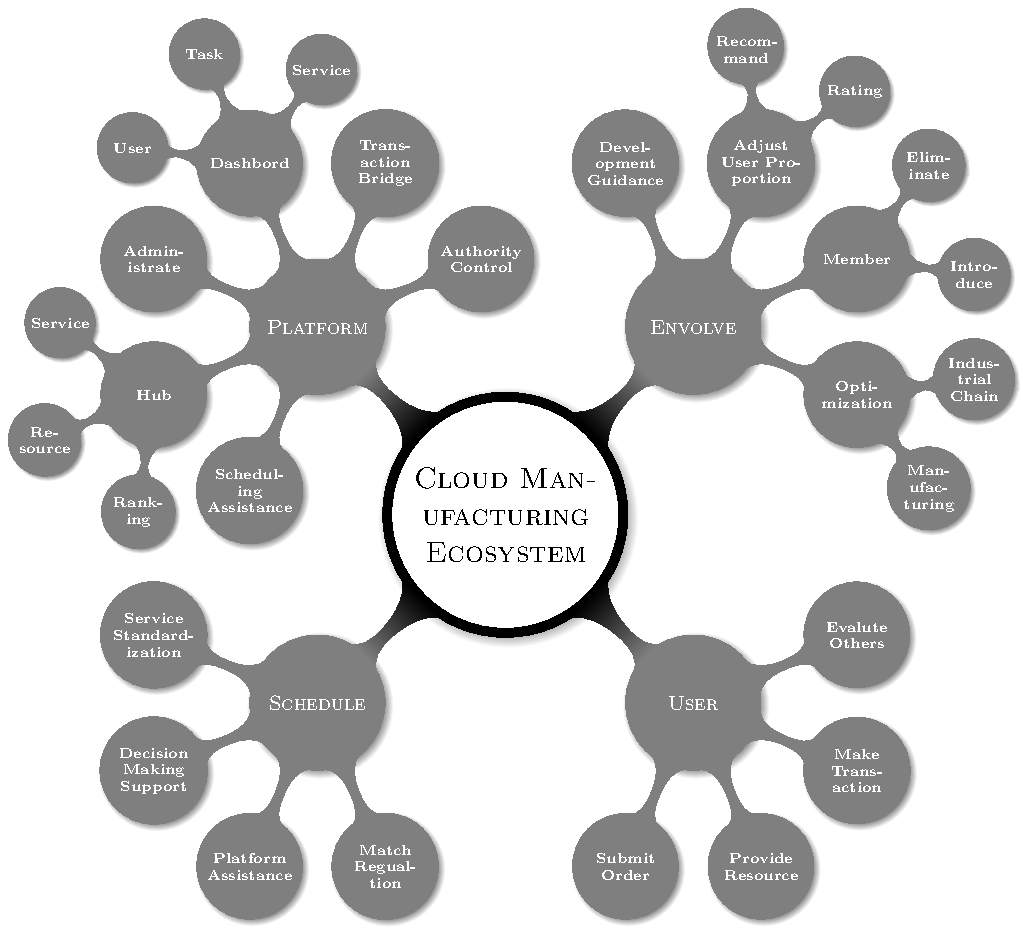
\includegraphics[height=0.82\textheight]{figures/platformstruct.pdf}
	\caption{Principal Structure of Cloud Manufacturing Ecosystem}
	\end{figure}
}
\iffalse
\only<2>{
	\begin{figure}
	\centering
	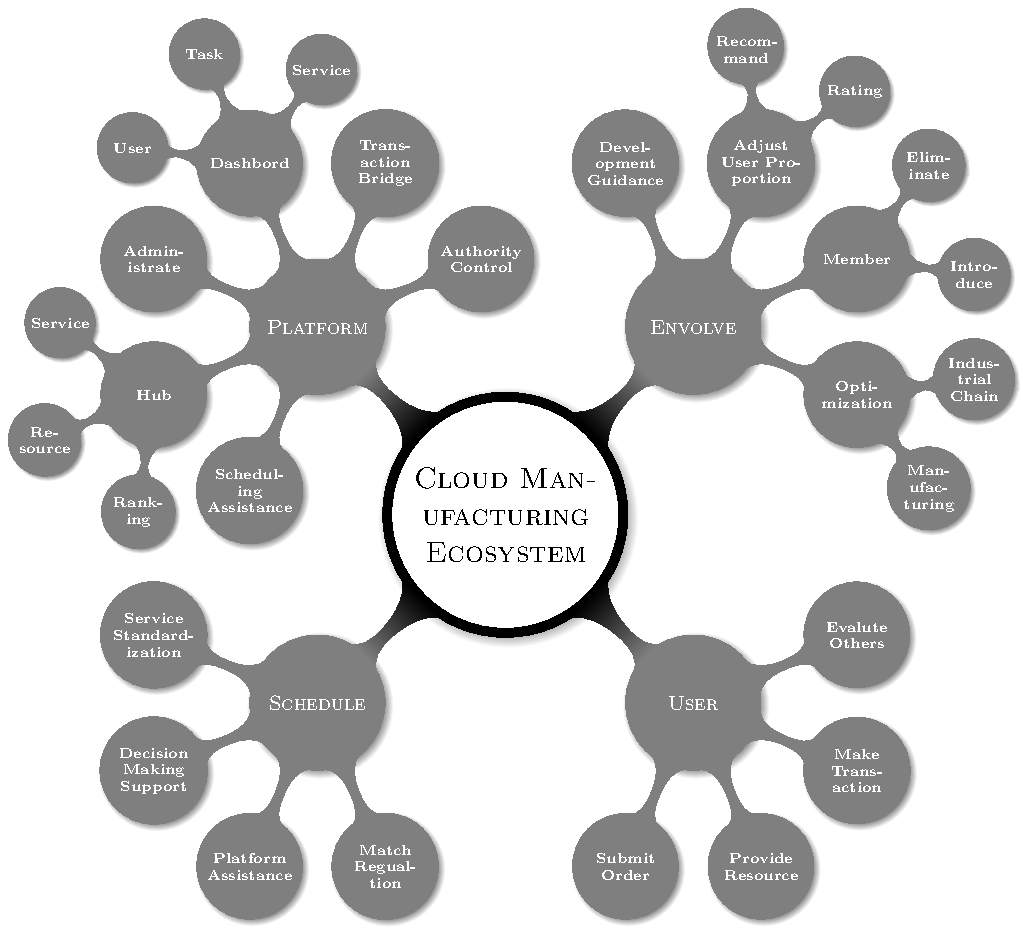
\includegraphics[height=0.82\textheight,viewport=40 0 500 250,clip=true]{figures/platformstruct.pdf}
	\end{figure}
}
\only<3>{
	\begin{figure}
	\centering
	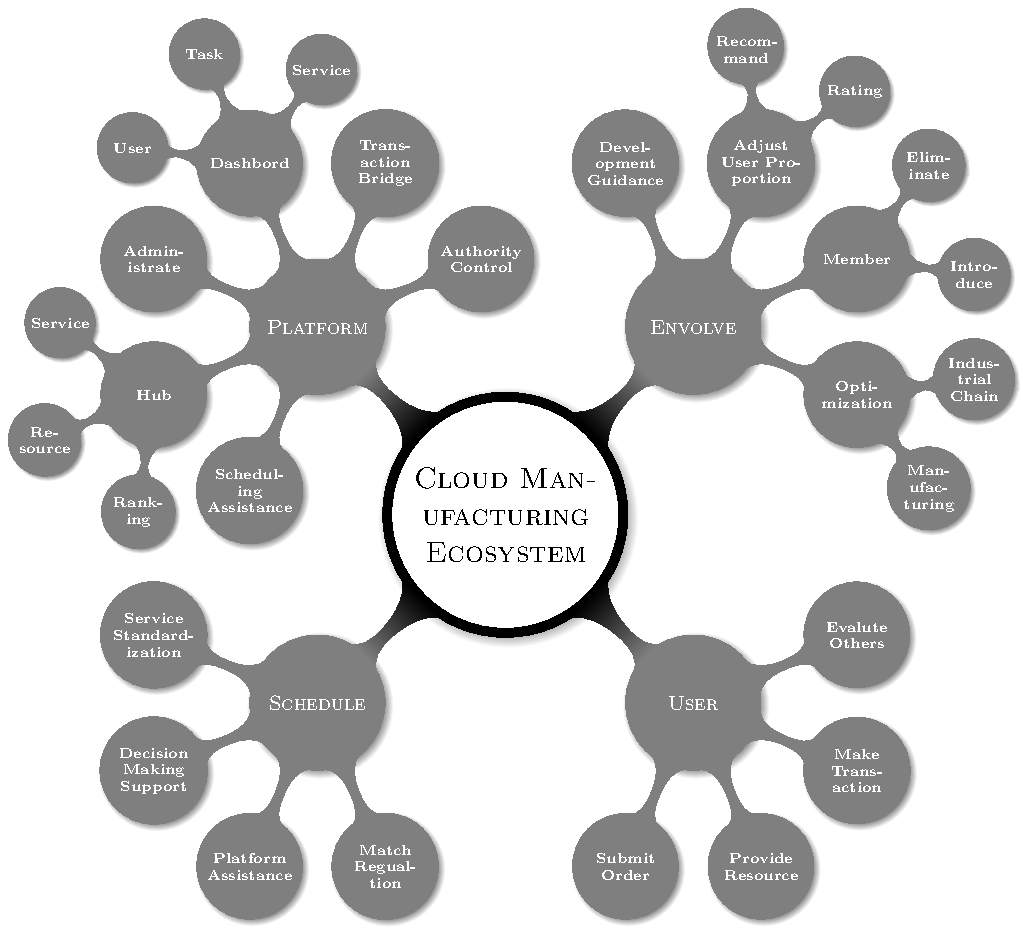
\includegraphics[height=0.82\textheight,viewport=0 160 500 450,clip=true]{figures/platformstruct.pdf}
	\end{figure}
}
\fi
\end{frame}

\begin{frame}{Service Standardization}{Cloud Manufacturing}
\begin{figure}
\centering
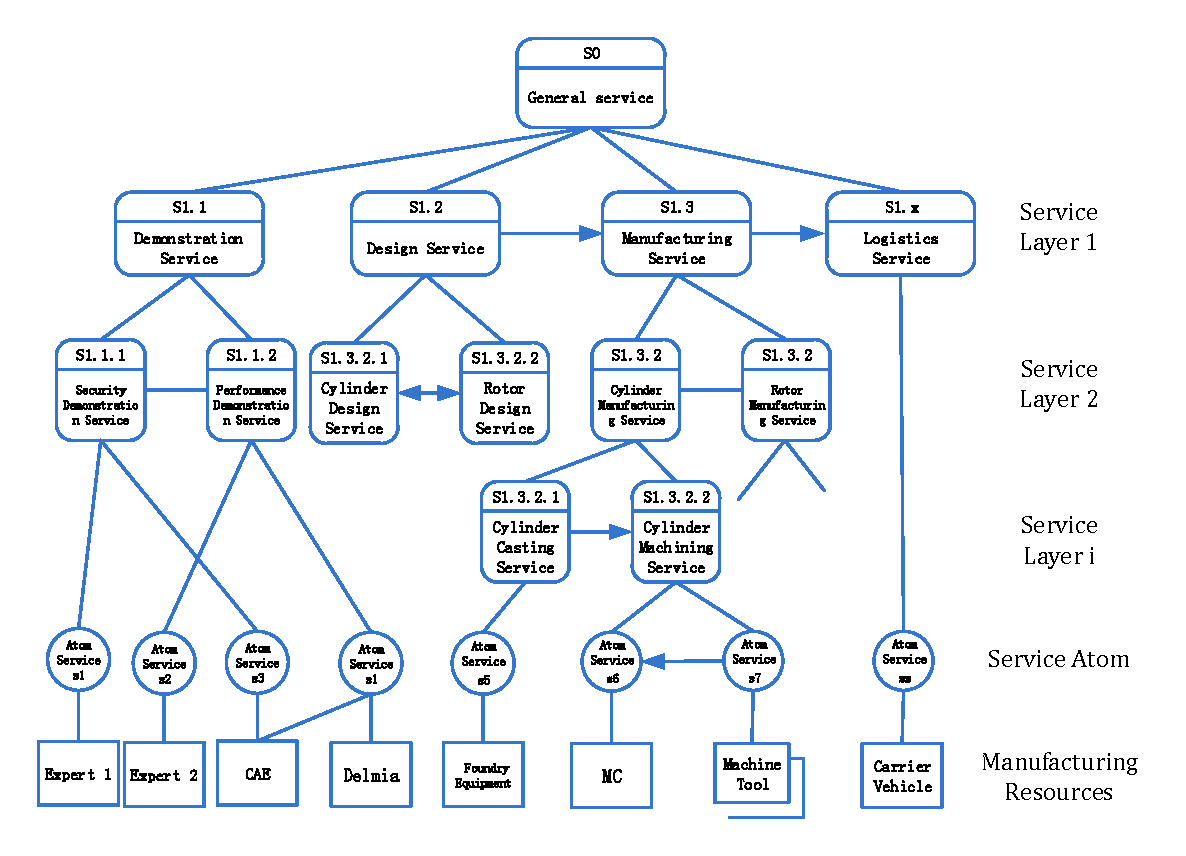
\includegraphics[height=0.85\textheight]{figures/boss.pdf}
\caption{Standard Service Tree Illustration}
\end{figure}
\iffalse
\onslide<+->{
	Cloud Manufacturing Ecosystem provides a platform which distributed manufacturing resources/orders gathered as resources/orders hub.
}
\onslide<+->{
	\begin{block}{Related Methods}
	\begin{itemize}
	\item Resource Virtualization
	\item Construct Virtual Resource into Service Unit
	\item Service Standardization
	\item Order Decomposition into Tasks
	\end{itemize}
	\end{block}
}
\fi
\end{frame}

\subsection{Roles}
\begin{frame}{Usual Names}{Roles}
\onslide<+->{\small
	\begin{description}
	\item[User] The main role in Cloud Manufacturing, usually acts as a Seller or a Buyer;
	\item[Seller] The temporary role in a transaction, which provides the allocated part of manufacturing service;
	\item[Buyer] The temporary role in a transaction, which submits the allocated part of manufacturing task;
	\item[Administrator] The role that gets the work for the operation and maintenance of the platform.
	\end{description}
}
\onslide<+->{
\begin{table}[htbp]
  \centering\scriptsize
    \begin{tabular}{lcc}
    \toprule
        &  Seller & Buyer  \\
    \midrule
    Generalized User & $\surd$ & $\surd$  \\
    Enterprise User & $\surd$ &  \\
    Customer User& & $\surd$ \\
    \bottomrule
    \end{tabular}%
\end{table}
}
\end{frame}

\subsection{Operating Model}
\begin{frame}{Overview}{Operating Model}
\only<1>{The style the Cloud Manufacturing Ecosystem appears mainly depends on the way the operating model takes, therefore, research on features and issues in the Ecosystem would be taken within the scope of operating model we are going to set up in:
\begin{block}{Operating Model Components}
\begin{itemize}
\item Order Flow
\item User Rank
\item Platform
\end{itemize}
\end{block}}
\only<2>{\begin{figure}
\tiny\centering\resizebox{\textwidth}{!}{
% !TEX root = flow_head.tex
\begin{tikzpicture}[
 >=triangle 60,              % Nice arrows; your taste may be different
 start chain=going right,    % General flow is top-to-bottom
 node distance=12em and 3em, % Global setup of box spacing
 every join/.style={norm},   % Default linetype for connecting boxes
]
% ------------------------------------------------- 
% A few box styles 
% <on chain> *and* <on grid> reduce the need for manual relative
% positioning of nodes
\tikzset{
  every node/.style={rectangle split, rectangle split parts=2, rectangle split horizontal, rectangle split part fill={lccong!25, yellow!10}, draw, anchor=center, minimum height=9em, on chain, on grid, text width=2em},
  base/.style={draw, on chain, on grid, align=center, minimum height=4ex},
  proc/.style={base, rectangle, text width=8em},
  Arrow/.style={thick, decoration={markings,mark=at position
   1 with {\arrow[semithick]{open triangle 60}}},
   double distance=1.4pt, shorten >= 5.5pt,
   preaction = {decorate},
   postaction = {draw,line width=1.4pt, white,shorten >= 4.5pt},fill = lcnorm!25},
  test/.style={base, diamond, aspect=2, text width=5em},
  term/.style={proc, rounded corners},
  % coord node style is used for placing corners of connecting lines
  coord/.style={coordinate, on chain, on grid, node distance=6mm and 25mm},
  % nmark node style is used for coordinate debugging marks
  nmark/.style={draw, cyan, circle, font={\sffamily\bfseries}},
  % -------------------------------------------------
  % Connector line styles for different parts of the diagram
  norm/.style={->, draw, lcnorm, thick},
  free/.style={->, draw, lcfree},
  cong/.style={->, draw, lccong},
  it/.style={font={\small\itshape}},
  tw/.style={text width=9.5em},
  th/.style={text width=2em}
}

\newcommand{\one}[1]{\nodepart[th]{one}\rotatebox{90}{\bf\shortstack{#1}}}
\newcommand{\two}{\nodepart[tw]{two}}

\node (n1)
{	
	\one{Service\\ Provide}
	\two
	\begin{inparaenum}
	\item 1.Submit Resources\\
	\item 2.Construct Resources into Services\\
	\item 3.Service Standardization
	\end{inparaenum}
};

\node[join] (n2) 
{
	\one{Task\\ Matching}
	\two
	\begin{inparaenum}
	\item 1.Recommanded Tasks\\
	\item 2.Order Acception \\
	\item 3.Decision
	\end{inparaenum}
};

\node[join] (n3)
{
	\one{Manufacturing\\ \& Schedule}
	\two
	\begin{inparaenum}
	\item 1.Manufacturing\\
	\item 2.Schedule Tasks\\
	\item 3.Outsourcing\\
	\item 4.Receive job pieces
	\end{inparaenum}
};

\node[below=of n3,join] (n4)
{
	\one{Delivery}
	\two
	\begin{inparaenum}
	\item 1.Deliver Completed job\\
	\item 2.Wait for Confirmation
	\end{inparaenum}
};

\node[below=of n2,join] (n5)
{
	\one{Mutual\\ Rating}
	\two
	\begin{inparaenum}
	\item 1.Rate Buyer\\
	\item 2.Receive Rate by Buyer\\
	\item 3.Change Rank\\
	\item 4.Change Recommendation
	\end{inparaenum}
};
\end{tikzpicture}}
\caption{Seller Flow in Operating Model}
\end{figure}}
\only<3>{\begin{figure}
\tiny\centering\resizebox{\textwidth}{!}{
% !TEX root = flow_head.tex
\begin{tikzpicture}[
 >=triangle 60,              % Nice arrows; your taste may be different
 start chain=going right,    % General flow is top-to-bottom
 node distance=12em and 3em, % Global setup of box spacing
 every join/.style={norm},   % Default linetype for connecting boxes
]
% ------------------------------------------------- 
% A few box styles 
% <on chain> *and* <on grid> reduce the need for manual relative
% positioning of nodes
\tikzset{
  every node/.style={rectangle split, rectangle split parts=2, rectangle split horizontal, rectangle split part fill={lccong!25, yellow!10}, draw, anchor=center, minimum height=9em, on chain, on grid, text width=2em},
  base/.style={draw, on chain, on grid, align=center, minimum height=4ex},
  proc/.style={base, rectangle, text width=8em},
  Arrow/.style={thick, decoration={markings,mark=at position
   1 with {\arrow[semithick]{open triangle 60}}},
   double distance=1.4pt, shorten >= 5.5pt,
   preaction = {decorate},
   postaction = {draw,line width=1.4pt, white,shorten >= 4.5pt},fill = lcnorm!25},
  test/.style={base, diamond, aspect=2, text width=5em},
  term/.style={proc, rounded corners},
  % coord node style is used for placing corners of connecting lines
  coord/.style={coordinate, on chain, on grid, node distance=6mm and 25mm},
  % nmark node style is used for coordinate debugging marks
  nmark/.style={draw, cyan, circle, font={\sffamily\bfseries}},
  % -------------------------------------------------
  % Connector line styles for different parts of the diagram
  norm/.style={->, draw, lcnorm, thick},
  free/.style={->, draw, lcfree},
  cong/.style={->, draw, lccong},
  it/.style={font={\small\itshape}},
  tw/.style={text width=9.5em},
  th/.style={text width=2em}
}

\newcommand{\one}[1]{\nodepart[th]{one}\rotatebox{90}{\bf\shortstack{#1}}}
\newcommand{\two}{\nodepart[tw]{two}}

\node (n1)
{	
	\one{Submit\\ Order}
	\two
	\begin{inparaenum}
	\item 1.Original\\
	\item 2.Outsourcing
	\end{inparaenum}
};

\node[join] (n2) 
{
	\one{Task\\ Construct}
	\two
	\begin{inparaenum}
	\item 1.Order Decomposition\\
	\item 2.Task Merging\\
	\item 3.Task Splitting
	\end{inparaenum}
};

\node[join] (n3)
{
	\one{Service\\ Matching}
	\two
	\begin{inparaenum}
	\item 1.Recommandation\\
	\item 2.Service Selection\\
	\item 3.Seller's Rank
	\end{inparaenum}
};

\node[below=of n3,join] (n4)
{
	\one{Confirm\\ by Seller}
	\two
	\begin{inparaenum}
	\item 1.Accept Tasks\\
	\item 2.Check Due-date\\
	\item 3.Buyer Rank
	\end{inparaenum}
};

\node[below=of n2,join] (n5)
{
	\one{Wait for\\ Delivery}
	\two
	\begin{inparaenum}
	\item 1.Wait the Seller\\
	\item 2.Confirm the Prouct\\
	\item 3.Pay for it
	\end{inparaenum}
};

\node[below=of n1,join] (n6)
{
	\one{Mutual\\ Rating}
	\two
	\begin{inparaenum}
	\item 1.Rate Seller\\
	\item 2.Change Rank\\
	\item 3.Affect Recommand
	\end{inparaenum}
};
\end{tikzpicture}}
\caption{Buyer Flow in Operating Model}
\end{figure}}
\end{frame}

\begin{frame}{Order Flow}{Operating Model}
\only<1>{Each order appears when Users make transaction in the platform, it might then go through different paths:
\begin{figure}
\tiny\centering
%\resizebox{\textwidth}{!}{% !TEX root = flow_head.tex
\begin{tikzpicture}[%
    >=triangle 60,              % Nice arrows; your taste may be different
    start chain=going below,    % General flow is top-to-bottom
    node distance=6mm and 60mm, % Global setup of box spacing
    every join/.style={norm},   % Default linetype for connecting boxes
    ]
% ------------------------------------------------- 
% A few box styles 
% <on chain> *and* <on grid> reduce the need for manual relative
% positioning of nodes
\tikzset{
  base/.style={draw, on chain, on grid, align=center, minimum height=4ex},
  proc/.style={base, rectangle, text width=8em},
  test/.style={base, diamond, aspect=2, text width=5em},
  term/.style={proc, rounded corners},
  % coord node style is used for placing corners of connecting lines
  coord/.style={coordinate, on chain, on grid, node distance=6mm and 25mm},
  % nmark node style is used for coordinate debugging marks
  nmark/.style={draw, cyan, circle, font={\sffamily\bfseries}},
  % -------------------------------------------------
  % Connector line styles for different parts of the diagram
  norm/.style={->, draw, lcnorm},
  free/.style={->, draw, lcfree},
  cong/.style={->, draw, lccong},
  it/.style={font={\small\itshape}}
}
% -------------------------------------------------
% Start by placing the nodes
\node [term] {Be Submitted};
\end{tikzpicture}
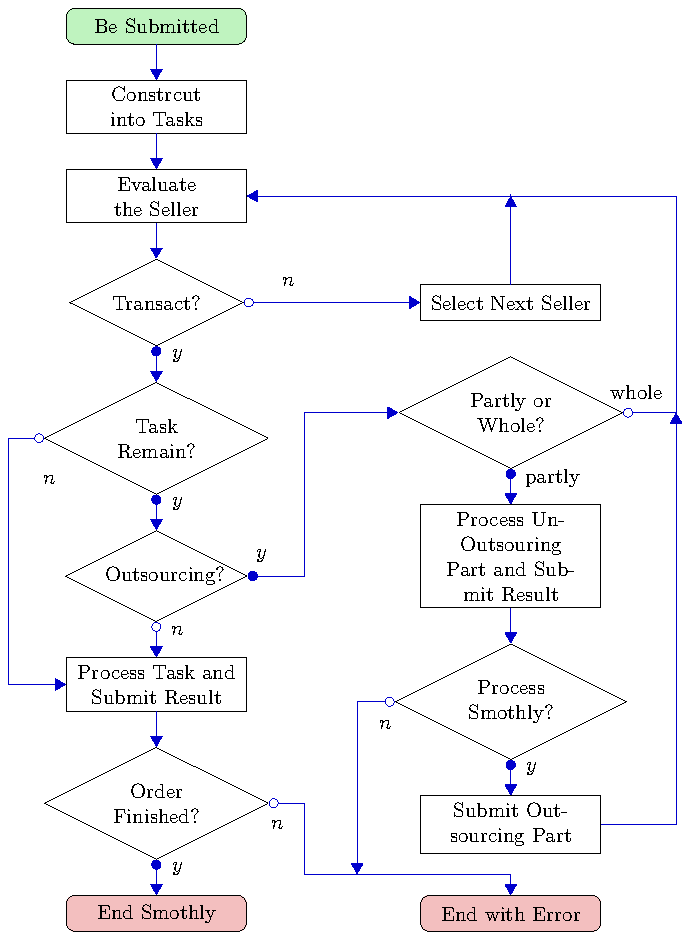
\includegraphics[height=0.9\textheight,angle=90]{figures/orderflow.pdf}
%}
\caption{Simple Flow Chart of Order}
\end{figure}
}
\end{frame}

\begin{frame}{User Rank}{Operating Model}
\onslide<+->{
The recommendation for tasks or services will be easily permissible, if their owner got high user rank,
the rank will change for their performance in every transaction }
\onslide<+->{
\begin{equation}
  \begin{cases}
      Rank_{[T+1]} = Rank_{[T]} + Gain - Lose, & T \geqslant 1\\
      Rank_{[0]} = Rank_{[init]}
  \end{cases}
\end{equation}
}
\onslide<+->{
	This equation set shows a simple user rank change style for both a seller and a buyer.
}
\end{frame}

\begin{frame}{Rank Change}{Operating Model}
\onslide<+->{
	\begin{figure}
	\centering
	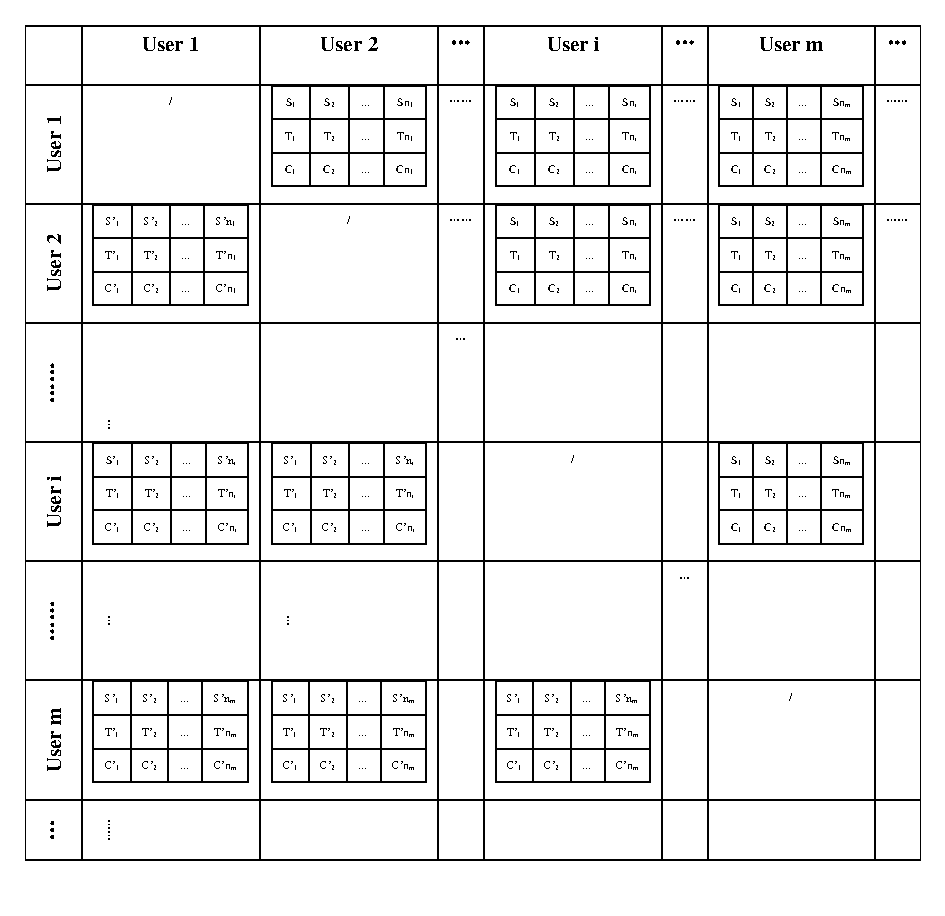
\includegraphics[trim=0 20 0 0,height=0.85\textheight]{figures/mutual.pdf}
	\caption{Mutual Evaluation for Input}
	\end{figure}
}
\end{frame}

\iffalse
\begin{frame}{Platform}{Operating Model}
\onslide<+->{
	Cloud Manufacturing Platform is mantained by Administrators with:
}
\onslide<+->{
	\begin{block}{Platform Maintenances}
	\begin{itemize}
	\item Decompose Orders into Tasks
	\item Construct Standard Services
	\item Introduce/Eliminate Users
	\item Distribute Permissions
	\item Adjust Resource Useage by Recommandations and Bonus
	\end{itemize}
	\end{block}
}
\end{frame}

\subsection{Data Science Tools}
\begin{frame}{Data Science Tools}
\onslide<+->{In such Cloud Manufacturing Operating Model, there comes massive amount of data:\begin{itemize}
  \item Transaction histroy;
  \item Ranking histroy;
  \item Status of resources, services, orders and tasks;
  \item Decision pattern and so on.
\end{itemize}}
\onslide<+->{
	A bunch of Data Science Tools can be helpful:
	\begin{block}{Useful Data Science Tools}
	\begin{itemize}
	\item Data Analysis (collection, cleaning, modeling\&algorithms)
	\item Data Warehousing
	\item Machine Learning
	\item Social Network Anaysis
	\end{itemize}
	\end{block}
}
\end{frame}
\fi
%\begin{frame}{Blocks}
%\begin{block}{Block Title}
%You can also highlight sections of your presentation in a block, with it's own title
%\end{block}
%\begin{theorem}
%There are separate environments for theorems, examples, definitions and proofs.
%\end{theorem}
%\begin{example}
%Here is an example of an example block.
%\end{example}
%\end{frame}

% Placing a * after \section means it will not show in the
% outline or table of contents.

% !TEX root = ../beamer.tex
\section{Services Scheduling}
\subsection{Standardization}
\begin{frame}{Services Scheduling}{Main}

\end{frame}
\subsection{Decision Making Support}
\begin{frame}{Services Scheduling}{Decision Making Support}

\end{frame}

\subsection{Matching Regualtion}
\begin{frame}{Services Scheduling}{Matching Regualtion}

\end{frame}

\subsection{Platform Assistance}
\begin{frame}{Services Scheduling}{Platform Assistance}

\end{frame}
% !TEX root = ../beamer.tex
\section{Manufacturing Ecosystem Envolving}
\subsection{Envolving Aim \& Main Factors}
\begin{frame}{Envolving Aim \& Main Factors}{Manufacturing Ecosystem Envolving}
\onslide<+->{The aim of envolving in the Ecosystem is to: \begin{itemize}
\item optimize the utilize of manufacturing resources
\item find the adaptive operating model for enterprises
\item filter out the underisable enterprises.
\end{itemize}}
\onslide<+->{
\begin{block}{Main Factors for Envolving}
\begin{itemize}
\item Rating Schema;
\item Recommand System and
\item Criterion of User Introduction and Elimination
\end{itemize}
\end{block}}
\end{frame}

\subsection{Rating Schema}
\begin{frame}{Rating Schema}{Manufacturing Ecosystem Envolving}
\onslide<+->{Rating user's rank is the base of Recommand System, so the rating schema should be designed. Most modern rating systems are derived from Elo's model:}
\onslide<+->{\begin{numcases}{}
E_A = \frac{1}{1+10^{\frac{R_B-R_A}{400}}} \\
R_A := R_A + K(S_A - E_A) \\
E_B = \frac{1}{1+10^{\frac{R_A-R_B}{400}}} \\
R_B := R_B + K(S_B - E_B)
\end{numcases}}
\end{frame}

\subsection{Recommand System}
\begin{frame}{Recommand System}{Manufacturing Ecosystem Envolving}
\onslide<+->{There are two scenarios in recommendation:
\begin{itemize}
\item Service Searching
\item Platform priority setting
\end{itemize}
}
\onslide<+->{
	Collaboration Filtering is popular method used in recommand system:
	\begin{equation}
	\begin{split}
	\min_{p_*,q_*,b_*} & \sum_{(u,i)\in\kappa}\left(r_{ui} -\mu - b_u - b_i - p^T_uq_i \right)^2 \\
		& + \lambda_3 \left( \|p_u\|^2 + \|q_i\|^2 + b_u^2 + b_i^2 \right)
	\end{split}
	\end{equation}
	\begin{numcases}{}
	\hat{r}_{ui} = b_{ui} + p^T_uq_i \\
	b_{ui} = \mu + b_u + b_i  \\
	\kappa =\{(u,i)|r_{ui} \text{is known}\} 
	\end{numcases}
}
\end{frame}

\subsection{User Introduction \& Elimination}
\begin{frame}{User Introduction \& Elimination}{Manufacturing Ecosystem Envolving}
\onslide<+->{
	Ecosystem envolving need a good user introduction and elimination method with:
}
\onslide<+->{
	\begin{block}{Envolving}
	\begin{itemize}
	\item Reinforcement Learning
	\item Control
	\end{itemize}
	\end{block}
}
\end{frame}

\subsection{Envision of the Ecosystem}
\begin{frame}{Envision}{After a long running time and the system seems stable}
\onslide<+->{
	With poper scheduling and envolving, Cloud Manufacturing Ecosystem running with a stable mode:
	\begin{block}{Stable System Envision}
	\begin{itemize}
		\item Less-Popular manufacturing services are utilized instead of idleness with Coupon
		\item Products are manufactured with appropriate resource
		\item High rank users in different type of manufacturing resource lead the industrial chain
		\item Good operating models appear and being refined with time goes by
	\end{itemize}
	\end{block}
}
\end{frame}
%% !TEX root = ../beamer.tex
\section*{Summary}

\begin{frame}{Summary}
  \begin{itemize}
  \item
    The \alert{first main message} of your talk in one or two lines.
  \item
    The \alert{second main message} of your talk in one or two lines.
  \item
    Perhaps a \alert{third message}, but not more than that.
  \end{itemize}
  
  \begin{itemize}
  \item
    Outlook
    \begin{itemize}
    \item
      Something you haven't solved.
    \item
      Something else you haven't solved.
    \end{itemize}
  \end{itemize}
\end{frame}





% All of the following is optional and typically not needed. 
\appendix
\section<presentation>*{\appendixname}
\subsection<presentation>*{bibliography}

\begin{frame}[allowframebreaks]
  \tiny
  \frametitle<presentation>{bibliography}
\nocite{*}    
\bibliography{references}
\end{frame}

\end{document}


